

\documentclass{article}
\usepackage{graphicx}
\usepackage{subcaption}
\usepackage{enumerate}
\usepackage{amsmath}
\usepackage{multirow}
\usepackage{bm}
\usepackage[ruled,linesnumbered]{algorithm2e}

\def\T{\mathrm{T}}


\title{Greedy-based RBS maximum allowable current calculation method} % #TODO: 修改标题
\author{3057761608 }
\date{March 2023}

\begin{document}

\maketitle

\begin{abstract}
    Reconfigurable Battery Systems (RBSs) offer a promising alternative to traditional battery systems, which are limited by their reliance on the worst-performing cell. 
    RBSs can dynamically adjust the circuit configuration to optimize battery cell charging and discharging strategies. 
    However, due to their reconfigurability, RBSs require new performance indicators to evaluate their performance.
    This paper proposes a method to estimate the Maximum Allowable Current (MAC), a crucial indicator to evaluate RBS performance. 
    The method employs a greedy algorithm based on a graph model and an equivalent circuit model. 
    By searching for the shortest path for battery cells to connect to the main circuit in the graph model, a greedy search strategy is provided for the equivalent circuit model to describe the switch state variables.
    The effectiveness of this method is validated on RBS structures of different sizes and configurations.
    The results also show that the ratio of the output current to the maximum battery current could better reflect the structural performance of RBS than the output current alone.
\end{abstract}

\section{Introduction}

Battery Energy Storage Systems (BESSs) are widely used to store and supply high-quality electrical energy in various applications, such as electric vehicles and wind power turbines\cite{desiqueiraControlStrategySmooth2021,karandehTwoStageAlgorithmOptimal2019,yangBatteryEnergyStorage2018,choCommercialResearchBattery2015}.
Typically, a BESS consists of numerous battery cells that are interconnected by series-parallel circuitry to provide the required charge storage capacity and output voltage.
However, as the number of cells increases, the reliability of the system becomes a major concern.
The capacity and safety of the BESS are mainly determined by the least healthy battery cells, a phenomenon known as the cask effect.
Furthermore, the degradation of cells in poor condition is accelerated by multiple charge/discharge cycles, which can lead to early failure of the unhealthy cells\cite{yangUnbalancedDischargingAging2016,fengPropagationMechanismsDiagnosis2019}.
These concerns are particularly problematic for traditional BESSs with fixed circuitry, which limit their practicality.

\begin{figure}[htbp]
    \centering
    \begin{subfigure}[b]{0.15\textwidth}
        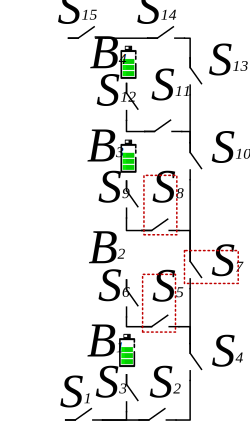
\includegraphics[width=\textwidth]{../attachments/arch-e.png}
        \caption{}
        \label{fig:arch-f}
    \end{subfigure}
    \hspace{0.05\textwidth}
    \begin{subfigure}[b]{0.3\textwidth}
        \includegraphics[width=\textwidth]{../attachments/arch-f.png}
        \caption{}
        \label{fig:arch-e}
    \end{subfigure}
    \begin{subfigure}[b]{0.3\textwidth}
        \includegraphics[width=\textwidth]{../attachments/arch-fe.png}
        \caption{}
        \label{fig:arch-ef}
    \end{subfigure}
    \caption{The RBS structure proposed by (a)Lawson\cite{lawsonSoftwareConfigurableBattery2012}, (b)Visairo\cite{visairoReconfigurableBatteryPack2008} and (c) synthesized from (a) and (b).}
    \label{fig:arch}
\end{figure}

Reconfigurable Battery System (RBS), which can dynamically switch between different circuit configurations as required, is expected to solve the above problem\cite{hanNextGenerationBatteryManagement2020a}. 
Unlike fixed BESSs, reconfigurable circuits use additional switches to change the series/parallel relationship between batteries.
Figure \ref{fig:arch} shows two proposed RBS structures (Figure \ref{fig:arch-e} and Figure \ref{fig:arch-f}), as well as a new structure (Figure \ref{fig:arch-ef}) synthesized from these two structures, all of which can dynamically adjust the connection of the battery as required.
For instance, in the structure shown in Figure \ref{fig:arch-e} when an unhealthy battery (the orange battery in the figure) exists in the system, the isolation of the battery can be achieved by closing the three adjacent switches marked in the figure and opening the switch below the battery to ensure the reliable operation of the system.
The structure in Figure \ref{fig:arch-f} is more flexible in terms of controlling system output.
Its switches can be used to connect the batteries in parallel or in series, thereby enabling the system to vary the system's output current or power.
By combining those two structures, cell isolation and output control can be easily achieved, as shown in Figure \ref{fig:arch-ef}. 
Therefore, compared with traditional fixed-structure battery systems, RBS has higher reliability and flexibility. 
However, due to the existence of more switches and more complex connection methods in RBS, there are more challenges in design, analysis, and control.


Maximum Allowable Current (MAC) is a critical parameter in the design and evaluation of reconfigurable battery systems (RBSs).
MAC specifies the maximum current that the RBS can output to external electrical equipment without exceeding a specified current limit for batteries.
This parameter is important for ensuring the safe and reliable operation of RBSs during normal operation and when failed batteries are isolated.
Despite its importance, there is currently no method in the literature on RBSs for calculating MAC, which poses a challenge for the design and evaluation of these systems.


The purpose of this paper is to propose a universal and effective method for calculating the Maximum Allowable Current (MAC) of RBS. 
To achieve this, models with RBS connection relationships and component status information are established, and then a greedy algorithm is used to search for MAC. This method has the following advantages:
1. It can effectively calculate MAC for RBSs with different sizes and structures.
2. A structural indicator is given to characterize the MAC of the structure, which is not affected by batteries and external circuits.
The paper is structured as follows: 
Section II presents the framework and details of the algorithm. 
In Section III, using a specific structure as an example, the application of the method is demonstrated, and the effectiveness of the method on RBS with different structures and sizes is verified. 
Finally, concluding remarks and future research directions are provided.

\section{Method}

\begin{figure}
    \centering
    \includegraphics[width=\textwidth]{../attachments/main-v4.png}
    \caption{Diagram of this method. 
        It includes a graph model and an equivalent circuit model based on the actual RBS.
        The shortest path of each battery is obstained from the graph model, and the voltage and current of the equivalent circuit model are calculated.
        By greedily searching for the combination of the shortest path, the MAC is calculated in the equivalent circuit model.
        } 
    \label{fig:main}
\end{figure}

Figure \ref{fig:main} shows the flowchart of our method.
Firstly, a graph model is abstracted from the actual RBS for finding the shortest path.
Then, an equivalent circuit model is established based on the graph model for solving the voltage and current in the circuit.
Finally, by greedily searching for the combination of the shortest path, the MAC is calculated in the equivalent circuit model.
\subsection{graph model and circuit model}

A typical RBS circuit is composed of battery cells and switches.
To establish a processable circuit, these components are transformed into ideal elements under reasonable assumptions.
The resulting circuit structure is then described in matrix form, and the related equations are provided.


The normal equivalent circuit for a battery consists of a voltage source in series with a resistor, and a capacitor in parallel with another resistor to simulate the polarization in batteries.
To calculate the MAC that can be stablely provided by RBS, only the steady-state behavior of the battery is considered in the model, and transient behavior is ignored.
Therefore, the battery $i$ is modeled as a constant voltage source $u_{b,i}$ in series with a resistor $r_{b,i}$.
And a binary variable $x_j$ is used to represent the state of switch $j$, where 0 and 1 indicate open and closed, respectively.
To simplify the calculation, a closed switch is considered as a resistor with a very small resistance value $r_s$, which are treated as zero in the final result.
In the following derivation, the product of the conductance $1/r_s$ and the variable $x_j$ is used to characterize the state of switch $j$.


A directed graph model $G(V,E)$ for the RBS is constructed in such a way that
\begin{enumerate}[(1)]
    \item Nodes: the vertex set $V={v_1,v_2,\cdots,v_N}$ represents the nodes connecting batteries and/or switches, where $v_1$ and $v_N$ represent the anode and cathode of the RBS respectively;
    \item Edges: the directed edge set $E$ represents the output circuit, $N_b$ batteries and $N_s$ switches, corresponding set $E_o$, $E_b$ and $E_s$. The external electrical equipment in the output circuit is treated as one directed edge $v_n \to v_1$. The direction of the edge representing a battery is set to be from the anode to the cathode. For the edges representing switches, their directions are marked from the low node to the the high node. A negative value for the voltage drop or current solved on the edge means that the actual direction is opposite to that initially specified.
\end{enumerate}


Based on the above directed graph which has $N$ nodes and $1+N_b+N_s$ directed edges (1 refers to the output circuit), its incidence matrix $\bm{A}_{N\times (1+N_b+N_s)}$ is defined as
\begin{align}\label{eq:A}
    a_{ij}=
    \begin{cases}
        1,  & \text{edge  $j$ leaves vertex $i$},\\
        -1, & \text{edge $j$ enters vertex $i$},\\
        0,  & \text{otherwise}.
    \end{cases}
\end{align}
Since each column of $\bm{A}$ sums to zero, the last line are deleted and the reduced incidence matrix $\bm{A}_{(N-1)\times(1+N_b+N_s)}$ are used in the following calculation.
By splitting $E$ into $\{E_o, E_b, E_s\}$, $A$ is rewritten as follows
\begin{equation}
    \bm{A} =
    \begin{bmatrix}
        \bm{A}_o & \bm{A}_b & \bm{A}_s
    \end{bmatrix}.
\end{equation}


$1+N_b+N_s$ edges' currents $\bm{I}_{(1+N_b+N_s)\times 1}$ and voltages $\bm{U}_{(1+N_b+N_s)\times 1}$, and $N-1$ nodes' voltages $\bm{U}_{n, (N-1)\times 1}$ have following relationships from Kirchhoffs law
\begin{align}\label{eq:Kirchhoffs_law}
    \begin{cases}
        \bm{A} \bm{I} = \bm{0}, \\
        \bm{U}        = \bm{A}^\T \bm{U}_n.
    \end{cases}
\end{align}
These directed edges are treated as generalized branches and expressed in matrix form as follows
\begin{equation}\label{eq:generalized_branches}
    \bm{I} = \bm{Y}\bm{X} \bm{U} - \bm{Y}\bm{X} \bm{U}_s +\bm{I}_s,
\end{equation}
where $\bm{I}$ and $\bm{U}$ are the column vectors about $1+N_b+N_s$ edges' current and voltage, respectively;
$\bm{U}_s$ and $\bm{I}_s$ denote the source voltage and source current of the generalized branches, respectively;
$\bm{Y}$ is the admittance matrix of the circuit, and $\bm{X}$ is the state matrix defined as
\begin{equation}\label{eq:X}
    \bm{X} = diag(
    1,
    \underbrace{1, \cdots, 1}_{N_b~\text{of}~1},
    \underbrace{1, 0 \cdots, 1}_{N_s~\text{of}~0/1}
    )
    =\begin{bmatrix}
        \bm{I} &\\
        & \bm{X}_s
    \end{bmatrix}.
\end{equation}


In addition to the equivalent circuit assumptions, we also assume that all batteries have the same internal resistance value $r_b$ and supply the same electric potential $u_s$ to simplify the model.
Then the output current $I_o$ and each battery's current $\bm{I}_b$ can be given by solving the simultaneous Equations \ref{eq:Kirchhoffs_law} and \ref{eq:generalized_branches} eventually.
Let
\begin{equation}\label{eq:Yn}
    \bm{Y}_n (\bm{X}) = \frac{1}{R_o} \bm{A}_o\bm{A}_o^\T + \frac{1}{r_b} \bm{A}_b\bm{A}_b^\T + \frac{1}{r_s}\bm{A}_s\bm{X}_s\bm{A}_s^\T,
\end{equation}
where $R_o$ is the equivalent resistance of the external circuit.
Then, if $\bm{Y}_n$ is an invertible matrix,
\begin{align}
    I_o(\bm{X})      & = \frac{u_b}{R_o r_b} \bm{A}_o^\T \bm{Y}_n^{-1}(\bm{X}) \bm{A}_b \bm{I}_{N_b\times 1};\label{eq:I_o}\\
    \bm{I}_b(\bm{X}) & = \frac{u_b}{r_b^2}[\bm{A}_b^\T \bm{Y}_n^{-1}(\bm{X}) \bm{A}_b\bm{I}_{N_b \times 1}  -r_b \bm{I}_{N_b \times 1}],\label{eq:I_b}
\end{align}
where $\bm{I}_{N_b\times 1}$ is a column vector with all terms being one.


Here, the ratio of $I_o$ and $\max (\bm{I}_b)$ is used to characterize the maximum allowable current for a given RBS architecture, denoted as $\eta$.
The discussion in the next section will show that the $\eta$ reflects the ability of the RBS architecture itself to deliver current, regardliess of the battery cells used by the RBS.
Finally the problem in RBS can be formulated as
\begin{align}
    & \max \eta \label{eq:max_eta}\\
    \mathrm{s.t.}\,\, & \eta = \frac{I_o}{\max (\bm{I}_b)}, \\
    & \max (\bm{I}_b) \leq I_m,
\end{align}
where $I_m$ is the maximum allowable current of the battery; $I_o$ and $\bm{I}_b$ can be calculated by Equations \ref{eq:I_o} and \ref{eq:I_b}.
However, it is difficult to solve \ref{eq:max_eta} directly because of the presence of matrix $\bm{Y}_n^{-1}$.
A greedy algorithm is proposed to solve this problem in the next subsection.


\subsection{greedy solution}

First, the battery $i$'s shortest path ($SP_i$) is given here.
When the battery $i$ is connected to the anode $v_1$ and the cathode $v_N$ of the RBS by the path $p$ in the graph model, the distance $\omega$ of $p$ is defined by the following equation:
\begin{equation}\label{eq:weight}
    \omega(p) = N_s \cdot n_b (p) + n_s (p),
\end{equation}
where $N_s$ is the total number of switches in the system; $n_b(p)$ and $n_s(p)$ are number of batteries and switches in the path $p$ respectively.
$SP_i$ is defined as the path with the minimum $\omega$ for battery $i$.
According to the definition, $SP_i$ gives the simplest strategy by which the control of battery $i$ is achieved with a minimum of switches while minimising the influence of other batteries.
From the perspective of series/parallel, the more batteries are connected into circuit via their $SP$s, the more batteries are connected in parallel.
Since batteries can provide more total output current when connected in parallel than in series, the algorithm greedily selects as many cells as possible to be connected into to the overall circuit via their $SP$s to obtain the MAC.
The dichotomy method is also performed to faster find the right number of $SP$s.


The pseudo-code of the algorithm is as follows:
\begin{algorithm}
    \caption{Get the max available currents of a certain RBS}\label{alg:eta_RBS}
    \KwData{Directed graph model $G(V,E)$ of the RBS}
    \KwResult{$\max \eta$}
    \For{$i \in E_b$}{
        $P_i \leftarrow \{path| \text{starts at $v_1$ and ends at $v_n$} \}$\;
        $SP_i \leftarrow p_i \text{ which has the minimum}~\omega(p_i)~\text{among all}~p_i \in P_i. $
    }
    get $\bm{A}$ by Equation \ref{eq:A}\;
    \While{not yet determine $\max \eta$ }
    {
        $N_{sel} \leftarrow \text{number of selected $SP$s calculated by dichotomy}$\;
        $C_b    \leftarrow \text{set of all combinations of $N_{sel} $~batteries from $N_b$}$\;
        \For{$c_b \in C_b$}{
            $\bm{x}_s \leftarrow \text{list of all switches' state: $x_s[j]=1$ if $ j \in \bigcup_{i\in c_b}SP_i $ else 0}$\;
            $\bm{X} \leftarrow diag[1,1,\cdots,1,\bm{x}_s] $\;
            get $\bm{Y}_n$ by Equation \ref{eq:Yn}\;
            \eIf{$\bm{Y}_n$ is invertible}{
            }{construct an effective solution}
            get $I_o$ by Equation \ref{eq:I_o}\;
            get $\bm{I}_b$ by Equation \ref{eq:I_b}\;
            \eIf{$\max(\bm{I}_b)\leq I_m$}{
                $\eta \leftarrow I_o/\max(\bm{I}_b)$\;
            }{break}
        }
    }
\end{algorithm}

\section{Examples}

This section verifies the effectiveness of the above model and algorithm on several structures.
Firstly, the detailed modeling and solving process of a specific RBS structure (proposed by \cite{visairoReconfigurableBatteryPack2008}) with four battery cells is given.
Then, the effectiveness is verified on RBSs with different structures and sizes.
This section also explains the advantages of using $\eta$ to characterize MAC.

\subsection{An specific example}

\begin{figure}[htbp]
    \centering
    \begin{subfigure}[b]{0.45\textwidth}
        \includegraphics[width=\textwidth]{../attachments/f4-phy.png}
        \caption{}
        \label{fig:f4-phy}
    \end{subfigure}
    \hspace{0.05\textwidth}
    \begin{subfigure}[b]{0.45\textwidth}
        \includegraphics[width=\textwidth]{../attachments/v3-new-main-2.png}
        \caption{}
        \label{fig:f4-gra}
    \end{subfigure}
    \\
    \begin{subfigure}[b]{0.45\textwidth}
        \includegraphics[width=\textwidth]{../attachments/f-dege-4-modify.png}
        \caption{}
        \label{fig:f4-circ}
    \end{subfigure}
    \hspace{0.05\textwidth}
    \begin{subfigure}[b]{0.45\textwidth}
        \includegraphics[width=\textwidth]{../attachments/f-dege-mac-4.png}
        \caption{}
        \label{fig:f4-mac}
    \end{subfigure}
    \caption{ 
        RBS structure proposed by Visairo\cite{visairoReconfigurableBatteryPack2008} with 4 batteries. 
        (a) Physical model, (b) graph model, (c) equivalent circuit model, and (d) results obtained by using the proposed method.
        The blue highlighted lines indicate the SPs. 
        The red highlighted lines indicate the open/close states of switches.
        }
    \label{fig:f4-all}
\end{figure}


The reconfigurable architecture proposed by Visairo et al.\cite{visairoReconfigurableBatteryPack2008} is shown in Figure \ref{fig:f4-phy}.
In this architecture, each cell is controlled by about 3 switches on average.
Excepted for two switches ($S_1$ and $S_{13}$ in Figure \ref{fig:f4-phy}) controlling the total circuit, the vertical switches (e.g. $S_2$ and $S_9$ in Figure \ref{fig:f4-phy}) allow the batteries to be directly connected to the main circuit, and the switches($S_6$ for example) in the diagonal direction can realize connecting the batteries in series.
Thus, it can dynamically change the output voltage and current as needed.
The architecture in Figure \ref{fig:f4-phy} only has 4 batteries, but in practice it can add new branches containing batteries and switches to deal with large-scale batteries\cite{kimDependableEfficientScalable2010}.


The graph in Figure \ref{fig:f4-gra} represents a graphical model based on the physical model(Figure \ref{fig:f4-phy}).
The model is presented in the form of a directed graph, capturing the connection relationship between the battery and switch in the circuit.
Vertex 1 and 12 represent the ancode and cathode of the RBS, respectively;
the remaining vertices represent the connection nodes between the batteries and switches.
Battery 1, 2, 3, and 4 are represented by green directed edges in the graph, while switches are represented by gray directed edges with opposite directions.
The external electrical appliance is considered as a directed edge from node 12 to node 1.
In the graph model, the directionality of the edges is strictly specified to ensure that there is no reverse flow of current in the battery and external electrical appliance.


According to Equation \ref{eq:weight}, the weight of the edge corresponding to the battery is the total number of switches, which is 13;
the weight of the edge corresponding to the switch is 1.
By setting the weight in this way, on the one hand, it avoids the simultaneous occurrence of multiple batteries in a single SP, weakening the influence between different batteries;
on the other hand, it minimizes the number of switches on the path, which means that only a few switches (i.e., the switches on the SP) need to be closed to connect the battery to the main circuit.
By using the depth-first search algorithm, the SP of battery 1 can be calculated as the node list $[1, 2, 3, 7, 11, 12]$, and the SPs of the other batteries are shown in Figure \ref{fig:f4-gra}.


The equivalent circuit model, as shows in Figure \ref{fig:f4-circ}, can be obtained based on the assumptions in Section II.
In this model, the batteries and switches are treated as branches, where the battery is regarded as a branch consisting of a voltage source $u_b$ in series with a resistor $r_b$, and the switch is regarded as a branch controlled by a state variable $x_s$ to short or open the circuit.
The branches are represented as direction edges, whose direction is from the node with the smaller number to the larger. 
When the computed current or voltage value is negative, it indicates that the direction of the battery or potential difference is opposite to the preset direction.
Based on the node-edge relationship in Figure \ref{fig:f4-circ}, the incidence matrix $\bm{A}$: can be obtained according to Equation \ref{eq:A}:
{\setlength{\arraycolsep}{2pt}
\begin{equation}
    \begin{array}{cc}
        &  \begin{array}{c c cccc ccccccccccccc} & e_o &e_{b1}  &e_{b2} & e_{b3} & e_{b4} & e_{s1} & e_{s2} & e_{s3} & e_{s4} & e_{s5} & e_{s6} & e_{s7} & e_{s8} & e_{s9} & e_{s10} & e_{s11} & e_{s12} & e_{s13} \end{array}\\
            \begin{array}{c} v_1\\v_2\\v_3\\v_4\\v_5\\v_6\\v_7\\v_8\\v_9\\v_{10}\\v_{11}\\v_{12}\end{array} & \left[
                    \begin{array}{c|cccc|ccccccccccccc}
                        -1  &  0  &  0  &  0  &  0  &  1  &  0  &  0  &  0  &  0  &  0  &  0  &  0  &  0  &  0  &  0  &  0  &  0\\
                        0  &  0  &  0  &  0  &  0  & -1  &  1  &  1  &  1  &  1  &  0  &  0  &  0  &  0  &  0  &  0  &  0  &  0\\
                        0  &  1  &  0  &  0  &  0  &  0  & -1  &  0  &  0  &  0  &  1  &  0  &  0  &  0  &  0  &  0  &  0  &  0\\
                        0  &  0  &  1  &  0  &  0  &  0  &  0  & -1  &  0  &  0  &  0  &  1  &  0  &  0  &  0  &  0  &  0  &  0\\
                        0  &  0  &  0  &  1  &  0  &  0  &  0  &  0  & -1  &  0  &  0  &  0  &  1  &  0  &  0  &  0  &  0  &  0\\
                        0  &  0  &  0  &  0  &  1  &  0  &  0  &  0  &  0  & -1  &  0  &  0  &  0  &  0  &  0  &  0  &  0  &  0\\
                        0  & -1  &  0  &  0  &  0  &  0  &  0  &  0  &  0  &  0  &  0  &  0  &  0  &  1  &  0  &  0  &  0  &  0\\
                        0  &  0  & -1  &  0  &  0  &  0  &  0  &  0  &  0  &  0  & -1  &  0  &  0  &  0  &  1  &  0  &  0  &  0\\
                        0  &  0  &  0  & -1  &  0  &  0  &  0  &  0  &  0  &  0  &  0  & -1  &  0  &  0  &  0  &  1  &  0  &  0\\
                        0  &  0  &  0  &  0  & -1  &  0  &  0  &  0  &  0  &  0  &  0  &  0  & -1  &  0  &  0  &  0  &  1  &  0\\
                        0  &  0  &  0  &  0  &  0  &  0  &  0  &  0  &  0  &  0  &  0  &  0  &  0  & -1  & -1  & -1  & -1  &  1\\
                    \end{array} \right]
    \end{array},
\end{equation}
}
where the rows correspond to vertexes in the graph model, and the first column, second to fourth columns, and last ten columns correspond to external electrical equipment, 4 batteries, and 13 switches, respectively.
According to the above classification of the columns, the matrix $\bm{A}$ can be divided into $\bm{A}_o$, $\bm{A}_b$, and $\bm{A}_s$.


The state matrix $\bm{X}$ is determined by the switches' state, that is, the specific configuration of the RBS.
For example, when switch
$S_1$, $S_2$, $S_3$, $S_4$, $S_5$, $S_9$, $S_{10}$, $S_{11}$, $S_{12}$ and $S_{13}$
are closed, and switch $S_6$, $S_7$ and $S_8$ are open, that is , battery $B_1$, $B_2$, $B_3$ and $_4$ are connected in parallel to supply power to the external circuit, the state matrix $\bm{X}$ is given by
\begin{equation}
    \bm{X} = diag(
    1,
    \underbrace{1,1,1,1}_{\text{batteries}},
    \underbrace{1,1,1,1,1,0,0,0,1,1,1,1,1}_{\text{switches}}
    ).
\end{equation}


When using the algorithm to solve the MAC, one may encounter the situation where the matrix $\bm{Y}_n$ is not full rank, and its inverse matrix cannot directly be obtained.
This is because so many switches are open that some branches with voltage sources are independent of the main circuit and form new circuits.
These circuits have infinite possible values for potential difference between them, since they are not connected to each other.
But the potential of the main circuit, which connects from node 1 to node 12 and completely determines the output, is certain and unique.
Therefore, the non-invertibility of $\bm{Y}_n$ will not affect the final solution.
Here, one can choose the solution where the potential at the node with the smallest number in the independent branch is 0.


\begin{table}[h]
    \caption{Detailed results of the proposed method for the RBS structure proposed by Visairo\cite{visairoReconfigurableBatteryPack2008} with 4 batteries, including the output current, current of each battery, and $\eta$.}
    \label{tab:1}
    \begin{tabular}{ccc}
        \hline
        output current $I_o$       & battery current $\bm{I}_b$       & $\eta$        \\
        \hline\\
        $\displaystyle\frac{4u_b}{4R_o + r_b}$ &  $\displaystyle\left[\frac{u_b}{4R_o + r_b},\frac{u_b}{4R_o + r_b},\frac{u_b}{4R_o + r_b},\frac{u_b}{4R_o + r_b}\right]$   & $4.00$ \\
        \\
        \hline
    \end{tabular}
\end{table}
The final calculation result of $\eta$ for the structure in Figure \ref{fig:f4-phy} is 4.
The corresponding currents of output and each battery are shown in Table \ref{tab:1}.
The corresponding switch control strategy is: $S_1$, $S_2$, $S_3$, $S_4$, $S_5$, $S_9$, $S_{10}$, $S_{11}$, $S_{12}$ and $S_{13}$ are closed (highlighted in red in Figure \ref{fig:f4-mac}), and $S_6$, $S_7$ and $S_8$ are open.
For this structure, when all batteries are connected to the main circuit through the switches in the vertical direction in Figure \ref{fig:f4-phy} and the batteries are connected in parallel, the output current is maximum, which is the sum of the currents of the four batteries.
The MAC of this structure is correctly estimated by our greedy algorithm.


From the specific results of the output current $I_o$ and battery currents $\bm{I}_b$, both are related to the battery voltage $u_b$, internal resistance $r_b$, and external circuit resistance $R_o$.
This means that even for the same structure, the output current will change when the external circuit  or the battery specifications  change.
By dividing the output current by the sum of the battery currents, the obtained $\eta$ does not include items affected by external circuit and batteries.
This characteristic is guaranteed by the linear nature of the RBS circuit.

\subsection{Different structures and sizes}

To further demonstrate the effectiveness of the models and algorithm, RBSs with different structures and sizes are considered.
On the one hand, the modeling and solving of the three battery structures in Figure \ref{fig:arch} are carried out, where the structure in Figure \ref{fig:arch-e} is proposed by Visairo\cite{visairoReconfigurableBatteryPack2008}, the structure in Figure \ref{fig:arch-f} is proposed by Lawson\cite{lawsonSoftwareConfigurableBattery2012}, and the structure in Figure \ref{fig:arch-ef} is a combination of the two. All three structures have 4 battery cells.
On the other hand, the modeling and solving of the battery structures proposed by Visairo\cite{visairoReconfigurableBatteryPack2008} with different numbers of battery cells (2, 4, and 6 cells) are also carried out.

The greedy algorithm provided accurate estimates of the structure MAC and generated safe and effective switch control strategies, as indicated by the results shown in Figure \ref{fig:d-structure} and \ref{fig:d-size}, where the highlighted red switches denote the closed positions.
Furthermore, the results about currents in Table \ref{tab:d-structure} and \ref{tab:d-size} show that the output currents are influenced by the external circuit resistance, battery potential, and internal resistance, but are linearly related to the battery currents, consistent with the conclusion about $\eta$ in the previous subsection.

\begin{figure}[htbp]
    \centering
    \begin{subfigure}[b]{0.45\textwidth}
        \includegraphics[width=\textwidth]{../attachments/e-dege-mac-4.png}
        \caption{}
        \label{fig:d-structure-f4}
    \end{subfigure}
    \hspace{0.05\textwidth}
    \begin{subfigure}[b]{0.45\textwidth}
        \includegraphics[width=\textwidth]{../attachments/f-dege-mac-4.png}
        \caption{}
        \label{fig:d-structure-e4}
    \end{subfigure}
    \hspace{0.05\textwidth}
    \begin{subfigure}[b]{0.45\textwidth}
        \includegraphics[width=\textwidth]{../attachments/e2f2-dege-mac.png}
        \caption{}
        \label{fig:d-structure-e2f2}
    \end{subfigure}
    \caption{
        The switches state when the output current is MAC on structure (a) proposed by Lawson\cite{lawsonSoftwareConfigurableBattery2012}, (b) proposed by Visairo\cite{visairoReconfigurableBatteryPack2008}, and (c) combining  Lawson's and Visairo's structure. 
        The red highlighted lines indicate the open/close states of switches.
        }
    \label{fig:d-structure}
\end{figure}

\begin{table}[h]
    \centering
    \caption{
        detailed results of the proposed method for the RBS with 4 batteries (a) proposed by lawson\cite{lawsonSoftwareConfigurableBattery2012}, (b) proposed by  visairo\cite{visairoReconfigurableBatteryPack2008} and (c) combining both  , including the output current, current of each battery, and $\eta$.}
    \label{tab:d-structure}
    \begin{tabular}{cccc}
        \hline
        structure &  output current $I_o$       & battery current $\bm{I}_b$       & $\eta$        \\
        \hline\\
        Lawson\cite{lawsonSoftwareConfigurableBattery2012} &  $\displaystyle\frac{u_b}{R_o + r_b}$ &  $\displaystyle\left[\frac{u_b}{R_o + r_b},0,0,0\right]$   & $1.00$ \\
        \\
        Visairo\cite{visairoReconfigurableBatteryPack2008} &  $\displaystyle\frac{4u_b}{4R_o + r_b}$ &  $\displaystyle\left[\frac{u_b}{4R_o + r_b},\frac{u_b}{4R_o + r_b},\frac{u_b}{4R_o + r_b},\frac{u_b}{4R_o + r_b}\right]$   & $4.00$ \\
        \\
        combining both &  $\displaystyle\frac{2u_b}{2R_o + r_b}$ &  $\displaystyle\left[\frac{u_b}{2R_o + r_b},\frac{u_b}{2R_o + r_b},0,0\right]$   & $2.00$ \\
        \\
        \hline
    \end{tabular}
\end{table}

\begin{figure}[htbp]
    \centering
    \begin{subfigure}[b]{0.45\textwidth}
        \includegraphics[width=\textwidth]{../attachments/f-dege-mac-2.png}
        \caption{}
        \label{fig:d-size-2}
    \end{subfigure}
    \hspace{0.05\textwidth}
    \begin{subfigure}[b]{0.45\textwidth}
        \includegraphics[width=\textwidth]{../attachments/f-dege-mac-4.png}
        \caption{}
        \label{fig:d-size-4}
    \end{subfigure}
    \hspace{0.05\textwidth}
    \begin{subfigure}[b]{0.45\textwidth}
        \includegraphics[width=\textwidth]{../attachments/f-dege-mac-6.png}
        \caption{}
        \label{fig:d-size-6}
    \end{subfigure}
    \caption{
        The switches state when the output current is MAC on structure proposed by Visairo\cite{visairoReconfigurableBatteryPack2008} with (a)2, (b)4 and (c) 6 batteries.  
        The red highlighted lines indicate the open/close states of switches.
        }
    \label{fig:d-size}
\end{figure}

\begin{table}[h]
    \caption{detailed results of the proposed method for the RBS proposed by visairo\cite{visairoReconfigurableBatteryPack2008} with (a)2, (b)4 and (c) 6 batteries , including the output current, current of each battery, and $\eta$.}
    \label{tab:d-size}
    \begin{tabular}{cccc}
        \hline
        size &  output current $I_o$       & battery current $\bm{I}_b$       & $\eta$        \\
        \hline\\
        2 &  $\displaystyle\frac{2u_b}{2R_o + r_b}$ &  $\displaystyle\left[\frac{u_b}{2R_o + r_b},\frac{u_b}{2R_o + r_b},\frac{u_b}{2R_o + r_b},\frac{u_b}{2R_o + r_b}\right]$   & $2.00$ \\
        \\
        4 &  $\displaystyle\frac{4u_b}{4R_o + r_b}$ &  $\displaystyle\left[\frac{u_b}{4R_o + r_b},\frac{u_b}{4R_o + r_b},\frac{u_b}{4R_o + r_b},\frac{u_b}{4R_o + r_b}\right]$   & $4.00$ \\
        \\
        6 &  $\displaystyle\frac{6u_b}{6R_o + r_b}$ &  $\displaystyle\left[\frac{u_b}{6R_o + r_b},\frac{u_b}{6R_o + r_b},\frac{u_b}{6R_o + r_b},\frac{u_b}{6R_o + r_b}\right]$   & $6.00$ \\
        \\
        \hline
    \end{tabular}
\end{table}

\section{Conclusion}

A graph model and a circuit model were developed, and a greedy strategy was employed to solve the MAC. 
The proposed method was tested on RBSs of varying structures and sizes. 
Additionally, an indicator, denoted by $\eta$ , was introduced to evaluate the performance of the RBS's output current. 
This work presents an effective approach for designing and evaluating the output current performance of RBS. 
Future research could focus on developing new performance indicators for evaluating RBS performance using the currents and voltages obtained by this method, as well as modifying the equivalent model of the battery to enable more accurate simulations of RBS, including transient analysis.

\bibliographystyle{ieeetr}
\bibliography{../attachments/my_ref}

\end{document}
